\section{Estimating Point Correspondence}%
\label{sec:perspective_projection}


\subsection{From Photometry to Geometry}%
\label{sub:from_photometry_to_geometry}


In the last sections, we discussed how points and lines are transformed
from 3D world coordinates to 2D image and pixel coordinates.\\

In practice, \textbf{we do not actually observe points or lines,
but rather brightness or color values} at the individual pixels.
In order to transfer from this photometric representation to a
geometric representation of the scene, one can identify points with
\textbf{characteristic image features} and try to associate these
points with corresponding points in the other frames.\\

The matching of corresponding points will allow us to infer 3D structure.
Nevertheless, one should keep in mind taht this approach is suboptimal:
\textbf{by selecting a small number of feature points from each image,
we throw away a large amount of potentially useful information contained
in each image}.
Yet retaining all image information is computationally challenging.
The selection and matching of a small number of feature points,
on the other hand, was shown to permit tracking of 3D objects from
a moving camera in real time.

\begin{figure}[h]
	\centering
	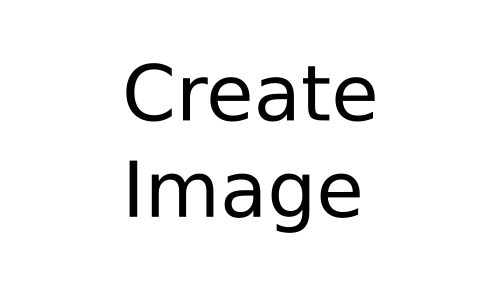
\includegraphics[width=\linewidth]{img/todo.png}
	\caption{Tracking of feature points}%
	\label{fig:traking_feature}
\end{figure}

To identify corresponding points in two or more images is one of the biggest
challenges in computer vision. Differences in point of view and
appearance can be challenging, due to materials, brightness, etc.
Small \textbf{baseline} make the tracking easier.\\

In what follows, we will assume that objects move rigidly.
In general, objects may also \textbf{deform non-rigidly}.
Moreover, there may be \textbf{partial occlusions}.
Quite often, points don't have correspondence in another image.
For example, in face tracking, teeth may disappear, smiles
may deform the face etc.\\

In point matching, one distinguishes two cases:

\begin{itemize}
	\item \textbf{Small deformation:} The deformation from one frame
		to the other is assumed to be (infinitesimally) small.
		In this case, the displacement from one frame to the othercan be estimated
		by classical \textbf{optic frow estimation}, for example using the methods
		of \textbf{Lucas/Kanade '81} or \textbf{Horn/Schunck '81}.
		These methods allow to model dense deformation fields (every pixel)
		but one can also track the displacement of a few feature points (faster).
	\item \textbf{Wide baseline stereo:} In this case the displacement is
		assumed to be large. A dense matching of all points to all is in general
		infeasible. Therefore, one typically selects a
		\textbf{small number of feature points} in each of the images
		and develops efficient methods to
		\textbf{find an appropriate pairing of points}.
\end{itemize}


\subsection{Small Deformation \& Optical Flow}%
\label{sub:small_deformation_optical_flow}


The transformation of all points of a rigidly moving objects is given by:
\[
	x_2 = h(x_1) = \frac{1}{\lambda_2(\bm{X})}
		(R \lambda_1(\bm{X}) x_1 + T)
\]
Locally this motion can be \textbf{approximated} in several ways.
\begin{itemize}
	\item Translation model: $h(x) = x + b$
	\item Affine model: $h(x) = Ax + b$
\end{itemize}
The 2D affine model can also be written with an offset $u$ as:
$h(x) = x + u(x)$ where:
\begin{align*}
	u(x) & = S(x)\ p \\
		 & = \begin{pmatrix}
				x & y & 1 & 0 & 0 & 0 \\
				0 & 0 & 0 & x & y & 1 \\
			\end{pmatrix}
			\tr{(p_1,p_2,p_3,p_4,p_5,p_6)}
\end{align*}

The \textbf{optic flow} refers to the apparent 2D motion field observable
between consecutive images of a video.
It is different from the motion of objects in the scene,
in the extreme case of motion along the camera axis, for example,
there is no optic frow, while on the other hand, camera rotation
generates an optic flow field event for entirely static scenes.\\

I 1981, two seminal works on optic flow estimation were published,
namely the works of \textbf{Lucas \& Kanade}, and of
\textbf{Horn \& Schunck}. Both methods have become very influential
with thousands of citations. They are complementary in the sense
that the Lucas-Kanade method generates, sparse flow vectors
under the assumption of constant motion in a local neighborhood,
whereas the Horn-Schunck method generates a dense flow field under
the assumption of spatially smooth flow fields.\\

Despite more than 30 years of research, the estimation of optic flow
fiels is still a highly active research direction.
Due to its simplicity, we will review the Lucas-Kanade method.


\subsection{The Lucas-Kanade Method}%
\label{sub:the_lucas_kanade_method}


\begin{itemize}
	\item \textbf{Brightness Constancy Assumption}:
		Let $x(t)$ denote a moving point at time $t$, and $I(x,t)$
		a video sequence, then:
		\[
			I(x(t),t) = \text{const.} \forall t,
		\]
		i.e.\ the brightness of point $x(t)$ is constant.
		Then the total time derivative must be zero:
		\[
			\frac{d}{dt} I(x(t),t)
			= \nabla \tr{I} \left(\frac{dx}{dt}\right)
				+ \frac{\partial I}{\partial t}
			= 0
		\]
		This constraint is often called the (differential)
		\textbf{optical flow constraint}. The desired local flow vector
		(velocity) is given by $v = \frac{dx}{dt}$.
		The fact that we can only recover the variation along
		the gradient is called in the literature,
		\textbf{the aperture problem}.

	\item \textbf{Constant motion in a neighborhood}:
		Since the above equation cannot be solved for $v$,
		one assumes that $v$ is constant over a neighborhood $W(x)$
		of the point $x$:
		\[
			\nabla \tr{I (x',t)} v + \frac{\partial I}{\partial t}(x',t)
				= 0,\quad \forall x'\ \in\ W(x)
		\]
		This assumption helps with the aperture problem.
\end{itemize}

The brightness is typically not exactly constant and the velocity
is typically not exactly the same for the local neighborhood.
\textbf{Lucas and Kanade (1981)} therefore compute the best velocity
vector $v$ for the point x by minimizing the \textbf{least squares error}.
\[
	E(v) = \int_{W(x)} | \nabla \tr{I(x',t)}v + I_t(x',t) | ^2 dx'
\]
Just a remark: nowadays, for precise optic flow computation,
one does not use this equation (not squared for example).
Expanding the terms and setting the derivative to zero one obtains:
\[
	\frac{dE}{dv} = 2 M v + 2 q = 0
\]
with
\[
	M = \int_{W(x)} \nabla I \tr{\nabla I} dx',\ \text{and} \
	q = \int_{W(x)} I_t \nabla I dx'
\]
If $M$ is invertible, then the solution is:
\[
	v = - \inv{M}q
\]
\begin{itemize}
	\item Translational motion: Lucas \& Kanade '81:
		\begin{align*}
			E(b) &= \int_{W(x)} | \tr{\nabla I} b + I_t |^2 dx' \\
			\frac{dE}{db} &= 0 \quad \implies b = \ldots
		\end{align*}
	\item Affine motion:
		\begin{align*}
			E(p) &= \int_{W(x)} | \tr{\nabla I(x')} S(x')p + I_t(x') |^2 dx' \\
			\frac{dE}{dp} &= 0 \quad \implies p = \ldots
		\end{align*}
		This energy $E(p)$ is quadratic in $p$ (a 6 parameters vector).
		We can essentially solve it doing the same as previously.
\end{itemize}

These techniques are easy to implement in theory.
However these should work only in the small deformation approximation (\roughly{} 1px).
This is very rarely the case with usual high resolution cameras.
One can use a \textbf{coarse to fine} algorithm to overcome this approximation.\\

In the formalism of Lucas and Kanade, one cannot always estimate a translational
motion. This problem is often referred to as the \textbf{aperture problem}.
It arises for example, if the region in the window $W(x)$ around the point $x$
has entirely constant intensity (for example a white wall),
because then $\nabla I(x) = 0$ and $I_t(x) = 0$ for all points in the window.\\

In order for the solution of $b$ to be unique, the \textbf{structure tensor}
\[
	M(x) = \int_{W(x)} \begin{pmatrix}
		I_x^2 & I_x I_y \\
		I_x I_y & I_y^2 \\
	\end{pmatrix} dx'
\]
needs to be invertible.
That means that we must have $\det M \neq 0$.
Or more realistically in practice, $M$ must not be \textbf{ill conditionned}.\\

If the structure tensor is not invertible but not zero,
then one can estimate the \textbf{normal motion} i.e.\ the motion
in direction of the image gradient.\\

In the regular case ($\det M \neq 0$), this leads to the following
simple feature tracker.
Feature tracking over a sequence of images can now be done as follows:
\begin{enumerate}
	\item For a given time instance $t$, compute at each point $x\in\Omega$
		the \textbf{structure tensor}
		\[
			M(x) = \int_{W(x)} \begin{pmatrix}
				I_x^2 & I_x I_y \\
				I_x I_y & I_y^2 \\
			\end{pmatrix} dx'
		\]
	\item Mark all points $x \in \Omega$ for which the determinant of $M$
		is larger than a threshold $\theta > 0$:
		\[
			\bm{\det M(x) \geq \theta}
		\]
	\item For all these points the local velocity is given by:
		\[
			\bm{b(x,t)} = - \inv{\bm{M(x)}} \begin{pmatrix}
				\int I_x I_t dx' \\
				\int I_y I_t dx' \\
			\end{pmatrix}
		\]
	\item Repeat the above steps for the points $x + b$ at time $t+1$.
\end{enumerate}


\subsection{Feature Point Extraction}%
\label{sub:feature_point_extraction}


\begin{figure}[h]
	\centering
	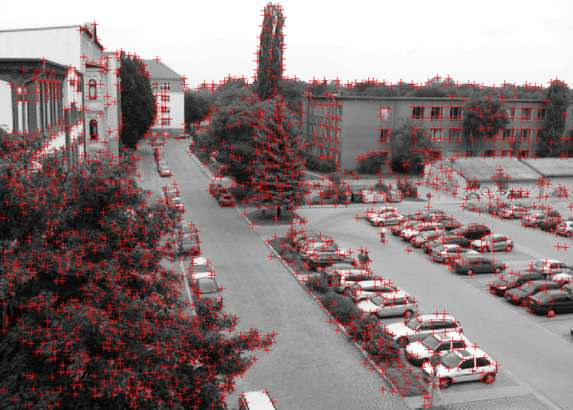
\includegraphics[width=\linewidth]{img/harris.jpg}
	\caption{Harris ``corner'' feature points.}%
	\label{fig:harris}
\end{figure}

Even $\det M(x) \neq 0$ does not guarantee robust estimates of velocity.
The inverse of $M(x)$ may not be very stable if, for example,
$M$ is ill conditionned (small determinant).\\

One of the classical feature detectors was proposed independently by
\textbf{F{\"o}rstner '84} and \textbf{Harris \& Stephens '88}
(Figure~\ref{fig:harris}). It is based on the \textbf{structure tensor}
\begin{align*}
	M(x) & \equiv G_{\sigma} * \nabla I \tr{\nabla I} \\
		& = \int G_{\sigma}(x-x') \begin{pmatrix}
			I_x^2 & I_x I_y \\
			I_x I_y & I_y^2 \\
		\end{pmatrix}
		(x') dx'
\end{align*}
where rather than simple summing over the window $W(x)$
we perform a summation weighted by a Gaussian $G$ of width $\sigma$.
The F\"orstner / Harris detector is given by:
\[
	\bm{C(x) = \det(M) + \kappa\ \text{trace}^2(M)}
\]
One selects points for which $C(x)>\theta$ with a threshold $\theta > 0$.


\subsection{Wide Baseline Matching}%
\label{sub:wide_baseline_matching}


Corresponding points and regions may look very different in different views.
In the case of \textbf{wide baseline matching}, large parts of the image
plane will not match at all because they are not visible in the other image.
In other words, while a given point may have many potential matches,
quite possibly it does not have any corresponding point in the other image.
Glass and in general, specular shiny objects really nasty to track.\\

One of the limitations of tracking features frame by frame is that
\textbf{small errors in the motion accumulate over time}
and the window gradually moves away from the point that was originally tracked.
This is known as \textbf{drift}.\\

A remedy is to match a given point back to the first frame.
This generally implies larger displacements between frames.
Two aspects matter when extending the above simple feature tracking
method to somewhat larger displacements:
\begin{itemize}
	\item Since the motion of the window between frames is
		(in general) no longer translational, one needs to
		\textbf{generalize the motion model} for the window $W(x)$,
		for example by using an \textbf{affine motion model}.
	\item Since the illumination will change over time
		(especially when comparing more distant frames), one can replace
		the sum-of-squared-differences by the
		\textbf{normalized cross correlation (NCC)} which is more
		\textbf{robust to illumination changes}.
\end{itemize}
\[
	NCC = \cos(v_1,v_2)
		= \frac{\inner{v_1}{v_2}}{|v_1|\ |v_2|}
\]
Where
\[
	v_i \equiv \text{vec}(I_i - \mean{I_i})
\]
$\mean{I_i}$ is the average intensity over the window $W(x)$.
By subtracting this average intensity, the measure becomes
\textbf{invariant to additive intensity changes} $I \rightarrow I + \gamma$.\\

Dividing by the intensity variances of each window makes the measure
\textbf{invariant to multiplicative changes} $I \rightarrow \gamma I$.\\

Let's look at the special case of \textbf{optimal affine transformation}.
The NCC can be used to determine the optimal affine transformation
between two given patches. Since the affine transformation is given
by $h(x) = A x + d$, we need to maximize the cross correlation
with respect to the $2\times2$-matrix $A$ and the displacement $d$:
\begin{align*}
	\widehat{A}, \widehat{d}
		& = \text{arg} \max_{A,d}\ NCC(A,D) \\
		& = \text{arg} \max_{A,d}\ \cos(v(x), v(Ax+d))
\end{align*}
This is not a convex cost function, so efficiently finding
appropriate optima is a challenge.\\

There exists many matching heuristics, some working better than others
depending on use cases. To evaluate the quality of point correspondence
algorithms, some have created \textbf{benchmarks}.
The challenge for creation of a good benchmark, is to get both
realistic images and accurate optic flow \textbf{ground truth}.
\begin{itemize}
	\item In the \textbf{Middlebury} benchmark, they superimposed
		very high frequency infrared pattern on images.
	\item In the \textbf{MPI Sintel} flow dataset is generated from
		an open source computer graphics short movie Sintel.
\end{itemize}
